%\documentclass[18pt,oneside,a4paper, titlepage]{article}

%\usepackage[hidelinks]{hyperref}
%\usepackage[pdftex]{graphicx}

%\begin{document}

\newpage
	\section{Architectural Design}
		\subsection{Overview}
				It has been adopted a four-tier architectural model, composed by thin client, web server, application server and database.\\ This architecture is the best choice for our system, even if it has some cons, such as the complexity of the structure and the difficulty of set up and maintenance, it still has several pros. For example, it guarantees increased performance, great flexibility, useful if there will be any future change concerning the architecture, and great security for each level, as there is no direct route from the web server to the database, with the introduction of a middle tier, which is essential as the application deals with several personal data.
\newpage
		\subsection{High level components and their interaction}
		% here you can introduce the high level components of your architecture (in our basic example in the slides about design you find these in slide 7) and describe the main interaction between them (no details here. You can say why some components talk to each other, why, if the communication is synchronous or asynchronous, any other info you think is useful at this point). 
			\vspace{1cm}
			\begin{figure}[h]
				\centering
				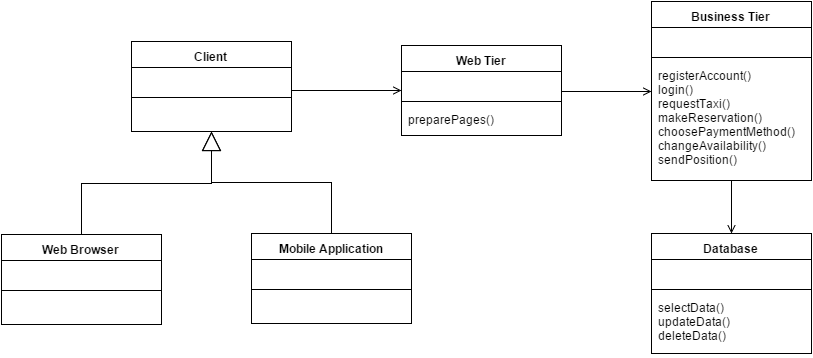
\includegraphics[scale=0.45]{HighLevelComp.png}
			\end{figure}
			\vspace{1cm}
			\begin{itemize}
				\item \textbf{Client tier}: this part runs on the client devices via a Web browser or the mobile application. It allows the users to insert and submit the data in the input forms, that are sent to the web tier. On the other hand, the taxi drivers can send information about their availability to the server and the application client monitors their GPS position in order to move the taxi drivers to another queue if they change their area. 
				\item \textbf{Web tier}: this part runs on the JEE server. It always listens to all the clients requests and forwards them to the business tier, if they need to be processed. It is the responsible for the creation of the faces and pages of the client interfaces with the data fetched from the business application.
				\item \textbf{Business tier}: this part runs on the JEE server, too. It contains the logical part of the application, collecting and managing the information of the other tiers. It analyses the data coming from the web tier and, according to the request, it modifies or asks for the required information stored in the database, then it is able to send the result to the web tier.  
				\item \textbf{EIS tier}: this part contains the database where all the application data are stored. It is not only accessed by the business tier, but also by the administrators, who can directly add a taxi driver account to the database. 
			\end{itemize}	
			
	\newpage
		\subsection{Component view}
		% here you have a refinement of what you have in Section 4.B and identify sub-components. For instance, the diagram in slide 6 could be a diagram showing a  component view
	\newpage	
		\subsection{Deployment view}
		% this is what you have in slide 8, that is, the identification of the artifact that need to be deployed to have the system working
	\newpage
		\subsection{Runtime view}
		%	You can use sequence diagrams to describe the way components interact to accomplish specific tasks typically related to your use cases
		% this is what you have in slide 9 plus sequence diagrams describing the way components behave in order to accomplish a certain activity
	\newpage
		\subsection{Component interfaces}
			% here you define the interfaces of your components, that is, which operations they offer to the external world, their meaning, any input and output parameter (name, possible set of values/type)
	\newpage
		\subsection{Selected architectural styles and patterns}
		%	Please explain which style/patterns you used, why and how
			
		\subsection{Other design decisions}
		% Section 4.G and 4.H are meant to include any explanation of the choices you have made and of their rationale. 		
%\end{document}